\section{Design}
\label{sec:design}

The application is designed using modern scalable technologies with clear separation of concerns across its various layers. 
The system is built upon a microservices [16] architecture pattern, enabling independent scaling and flexibility in deployment


\begin{figure}[!htbp]
\centering
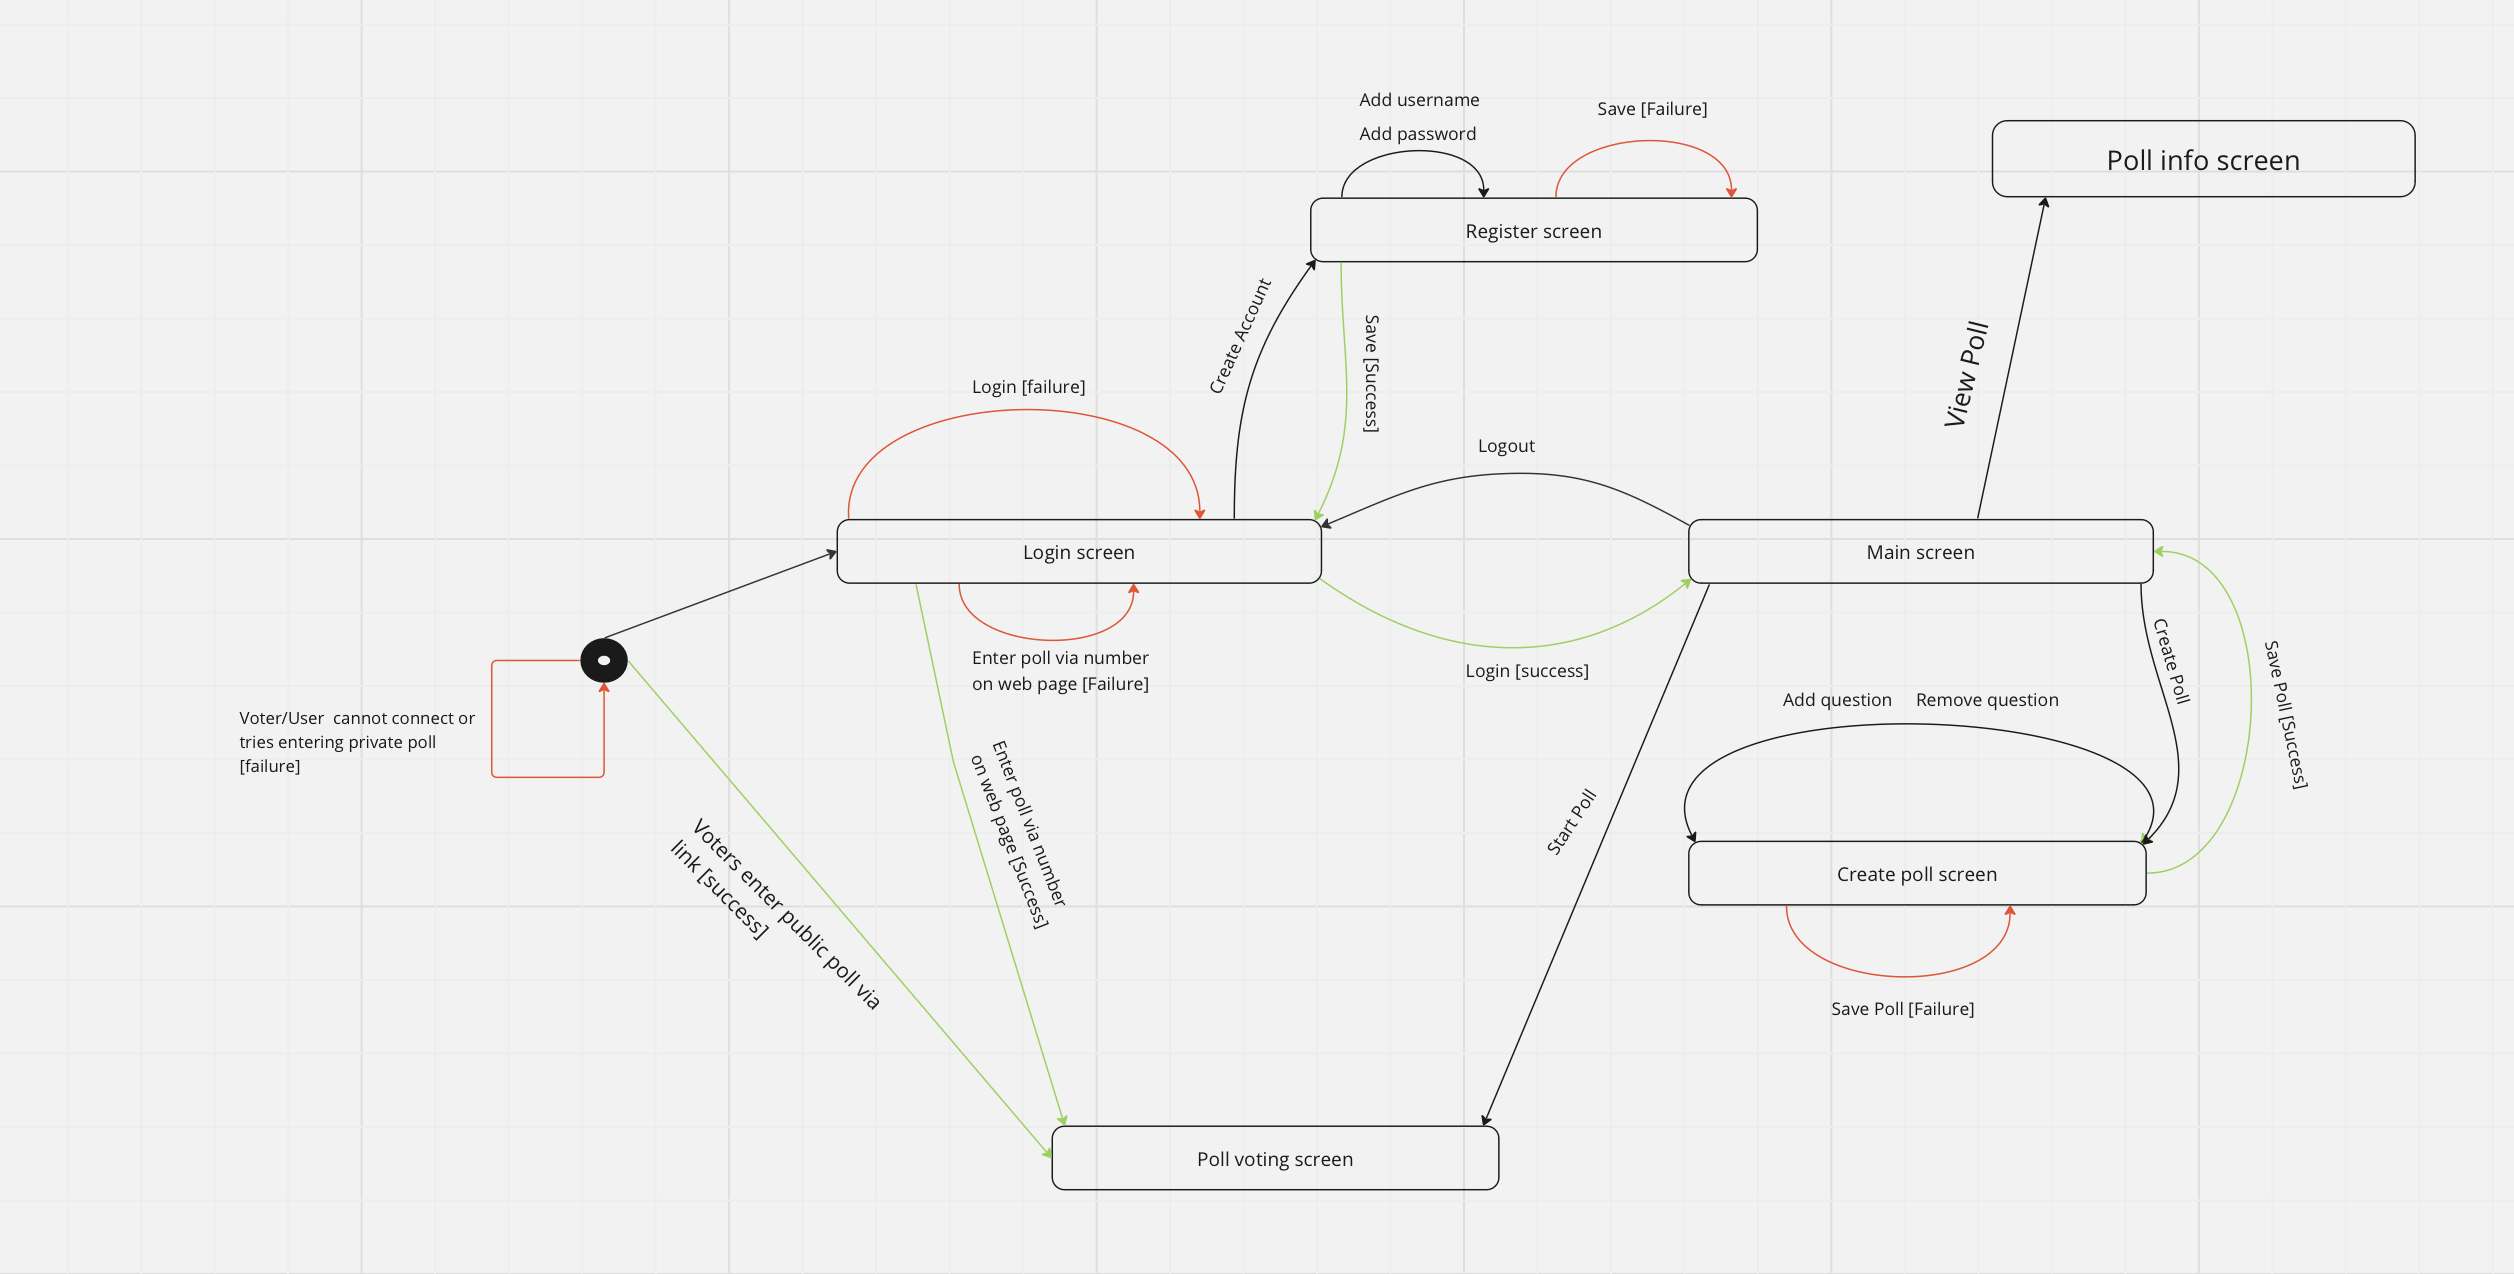
\includegraphics[width=\linewidth]{figs/ApplicationFlowDiagram.png}
\caption{Application flow diagram}
\label{fig:appflow}
\end{figure}

The application flow diagram, as seen in Figure~\ref{fig:appflow}, provides a high-level overview of the user's journey through the application. According to Lucidchart, process flow diagrams help to "show unnecessary steps, bottlenecks, and other inefficiencies" [5]. It begins with the Login screen, where users can either log in or register. In case of registration, the user is prompted to add a username and password before being redirected to the main screen upon successful account creation. The main screen serves as a navigation hub, allowing users to view polls, create new polls, or log out.

Upon selecting a poll, the user is taken to the Poll Voting screen, where they can cast their vote. Both successful and unsuccessful actions within the application are accounted for, with clear pathways leading the user to appropriate screens or error messages, ensuring a robust user experience. The diagram distinctly marks the paths taken during normal operation (success) and exceptions (failure), reflecting the applications error-handling capabilities.

The flow for creating a poll is similarly user-friendly, with the Create Poll screen allowing users to add or remove questions before saving. The user is provided with immediate feedback on the success or failure of their actions, with the system guiding them accordingly.

In addition to the primary user flows, the diagram also highlights potential failure states, such as login failures or issues entering private polls, indicating comprehensive error handling throughout the application.
    


\begin{figure}[!htbp]
\centering
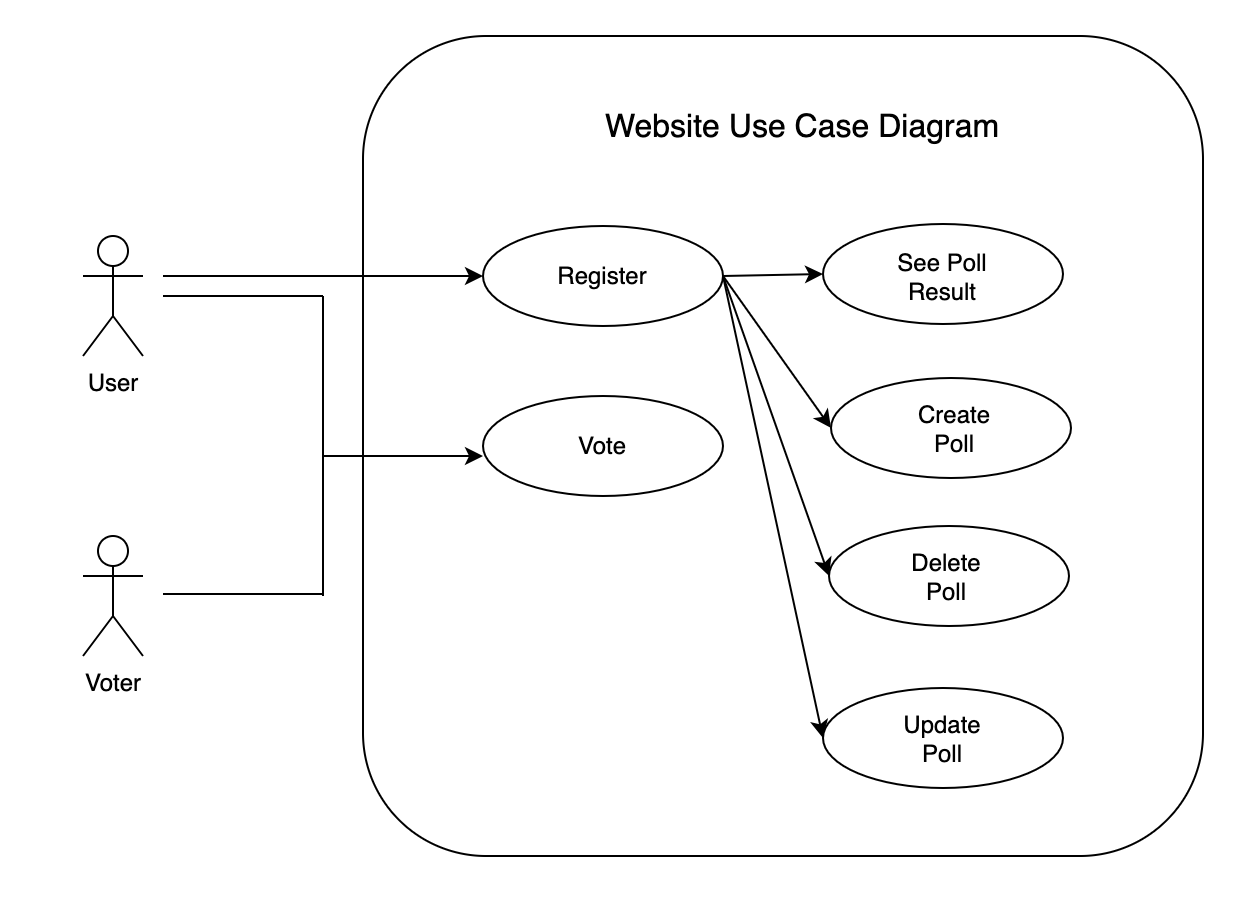
\includegraphics[width=0.5\linewidth]{figs/UserDiagram.png}
\caption{Website use case diagram}
\label{fig:userdiagram}
\end{figure}

Figure~\ref{fig:userdiagram} delineates the use case diagram for the website, detailing the interactions that both 'User' and 'Voter' actors have with the system. The 'User' actor, representing registered individuals, has the capabilities to register, vote, see poll results, create, delete, and update polls. The distinction between a general 'User' and a 'Voter' highlights the specialized role that a 'Voter' plays in the context of the application, primarily focused on the voting functionality. The use case diagram clearly identifies the system's boundary and the primary functions available to the users, providing a straightforward visualization of the different ways the users can interact with the system. "A key concept of use case modeling is that it helps us design a system from the end user's perspective" [6].


\begin{figure}[!htbp]
\centering
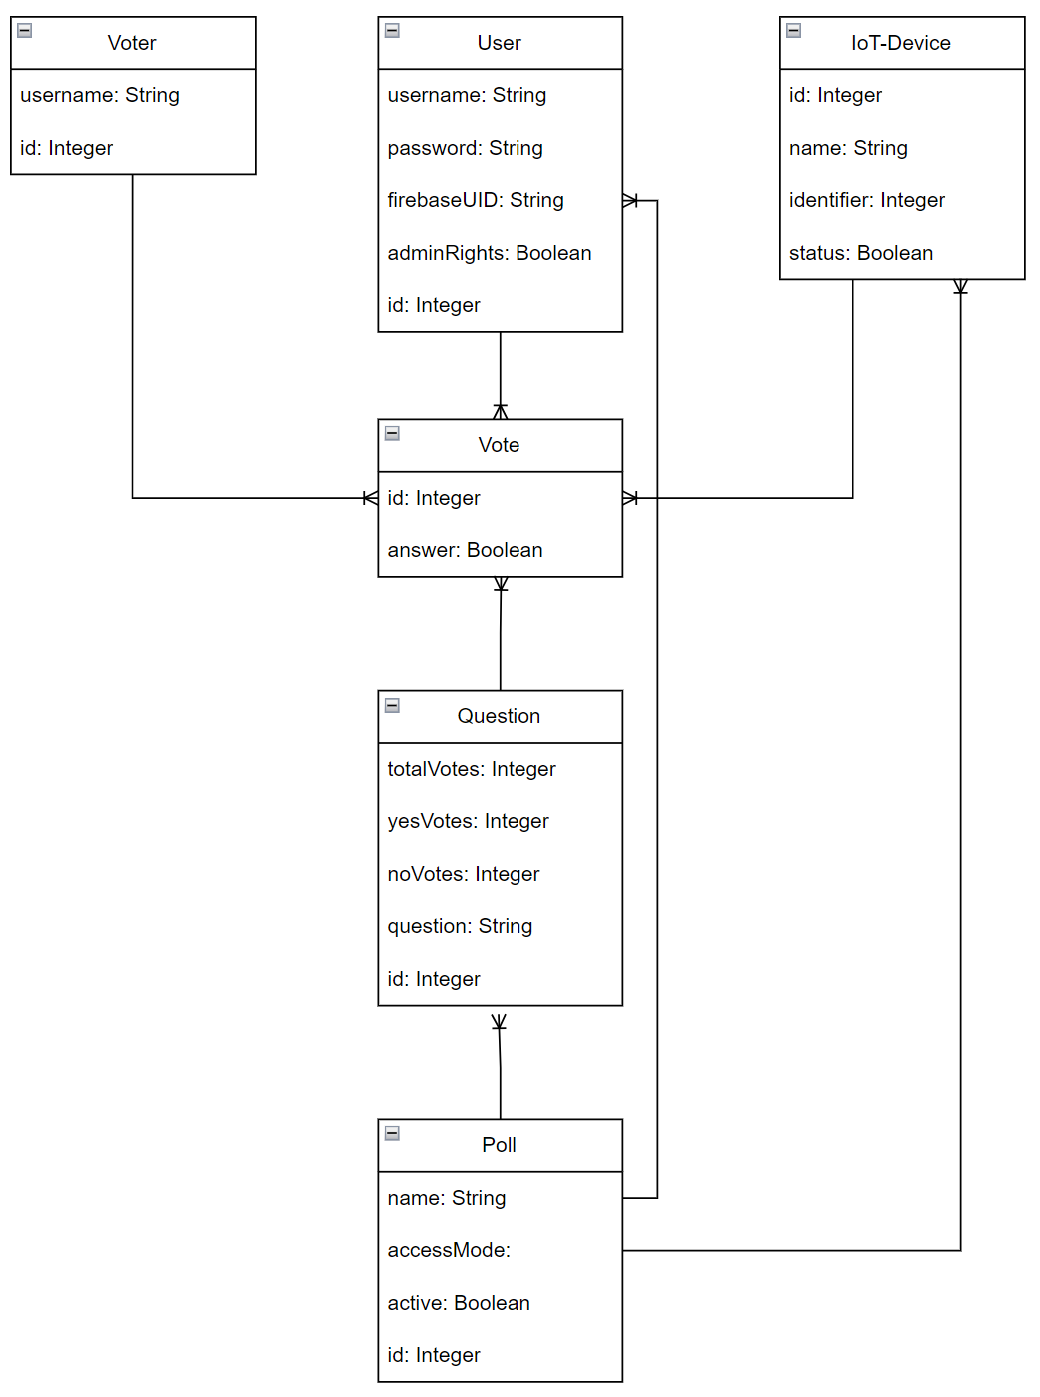
\includegraphics[width=0.4\linewidth]{figs/DomainModel.png}
\caption{Domain model}
\label{fig:domainmodel}
\end{figure}

Figure~\ref{fig:domainmodel} presents the domain model of the application, illustrating the primary entities and their relationships. "A domain model is a visual representation of real situation objects in a domain. A domain is an area of concern. It's used to refer to the area you are dealing with" [7]. The model defines a User entity with attributes for username, password, a unique Firebase user ID, administrative rights, and an identifier. This entity is central to the model and is associated with Voter, Vote, and IoT-Device entities.

The Voter is a specialized type of User, indicated by a shared id attribute, encapsulating only the necessary attributes for voting purposes, such as username and voter identifier. The Vote entity represents an individual vote, with a boolean answer attribute and a unique identifier, which is associated with a Question. Each Question contains attributes for the total number of votes, counts of yes and no votes, the text of the question, and an identifier.

The model also includes a Poll entity, which aggregates Questions. It has attributes for the poll name, access mode, an active status indicator, and an identifier. The IoT-Device entity represents devices that may interact with the system, characterized by an identifier, a name, another unique identifier, and a status boolean, which could be used for integrating IoT capabilities within the application.

This domain model serves as a blueprint for the systems structure, outlining the key data elements and their interconnections, which are crucial for understanding the relationships and data flow within the application.

\subsection{Design Patterns}

\subsubsection{Model-View-Controller (MVC)}

Our application employs the \textbf{Model-View-Controller (MVC)} design pattern, a paradigm for creating software with separated concerns, enhancing code reusability, and facilitating parallel development. The implementation of MVC within our voting application is outlined as follows:

\begin{description}
  \item[Model:] The model layer manages data and business logic. It encompasses domain entities corresponding to database tables, abstracting database access through Spring Data JPA with Hibernate. The models, defined as POJOs, encapsulate the application's data structures and business rules.
  
  \item[View:] Implemented using React.js, the View is a dynamic user interface for client-side interactions. Tailwind CSS is integrated for responsive and aesthetic styling. The frontend operates independently, interfacing with the server through API calls.
  
  \item[Controller:] Controllers in the `controller` package mediate between Model and View, handling HTTP requests with `@RestController` annotations. They direct user inputs to model operations and return appropriate responses, whether as rendered views or data payloads.
\end{description}
[8]

\paragraph{Advantages of MVC in Our Application:}
\begin{itemize}
  \item \textbf{Separation of Concerns:} MVC facilitates maintenance and scalability with its independent component operation.
  \item \textbf{Parallel Development:} Developers can work on the Model, View, and Controller concurrently, expediting development cycles.
  \item \textbf{Testability:} The separation allows for precise automated testing of business logic and user interfaces.
  \item \textbf{Adaptability:} Business logic or UI changes incur minimal impact on the overall architecture.
\end{itemize}

The MVC design pattern is integral to our application's design, ensuring a clean separation between user interface, business processing, and data management components, making the system robust, maintainable, and adaptable.[17]


\subsection{Architectural Layers Overview}

Our web application's architecture is thoughtfully organized into distinct layers, each serving a specific function, yet collectively contributing to a cohesive and efficient system.

The \textbf{Frontend Layer} features React.js for crafting the user interface, where components are meticulously designed to present the application's UI, facilitating data presentation and user interaction. Tailwind CSS is intricately used within this layer to style the React components, offering an enhanced user experience through a customized look and feel.

In the \textbf{Application Layer}, controllers, integral to our Spring Boot backend, manage HTTP requests. They process incoming data, trigger business logic, and return responses to the frontend, functioning as a pivotal connection point in the application flow.

The \textbf{Business Logic (Service) Layer} houses the core of our application's operations. It contains service classes that encapsulate the business rules and computations, bridging the gap between the presentation layer and the data access layer.

The \textbf{Data Access (Persistence) Layer} is key in managing data interactions. It comprises JPA repositories that abstract data layer operations and models that represent the application's business data, mapped to database tables. Hibernate, as our chosen JPA implementation, seamlessly handles the object-relational mapping, translating between the object model and the relational database representation.

Our \textbf{Configuration Layer} encompasses Spring configuration classes, which define beans and configure database and security settings, ensuring a robust and secure application infrastructure.

The \textbf{Database Layer} utilizes the H2 Database, an in-memory database ideal for persisting application data, accessed via the JPA repositories.

The \textbf{Authentication Layer} features Firebase Authentication services, crucial for user authentication. It is integrated into the application layer to secure endpoints and manage user sessions effectively.

The \textbf{Testing Layer} contains comprehensive unit and integration tests, ensuring each application component functions correctly both independently and collectively.

Finally, the \textbf{Build and Deployment Infrastructure} employs Gradle for dependency management, compilation, and packaging, while Docker is used to create a containerized application environment, promoting consistency across various development and production settings.

This modular layering not only enhances the maintainability and scalability of the application but also aligns perfectly with agile and DevOps practices, supporting continuous development and deployment.
